\chapter{Exploring The Model}
% This is where we describe our experiments. We insert plots, images, ....


Our initial aim was to explore various properties of the attractors in a Hopfield Network. We are interested in studying, testing or challenging several ideas about the neural network:
\begin{itemize}
 \item Clusters of attractors: We are interested to see how the Hopfield network behaves when learning similarly correlated patterns. This implies training the network with a cluster of attractors, which will lower the capacity of the network. We believe that basin sizes will get smaller as the patterns get closer to each other.
 \item Super-Attractors: Find out what happens if the network is trained several times with the same pattern. We believe this super-attractor will have a larger basin size compared to the other attractors.
 \item Convergence: We plan to train the network with different types of attractors and find out to which ones patterns tend to converge.
\end{itemize}


\section{Measuring the Basin Size}

 A large part of our experiments were thus dedicated to measuring basin sizes of different attractors, clusters of attractors and a newly introduced concept of \emph{Super-Attractors}.

 A recognised scientific method for calculating the basin size is the Storkey-Valabregue measurement:

 \begin{enumerate}
  \item Initially n = 1
  \item Choose an initial fixed point corresponding to a stored pattern \(\mu\)
  \item \label{itm:choose radius} Choose some initial normalised Hamming radius \(r=r_{0}\)
  \item Let the set A be all the states Hamming-distant \( nr \) from the fixed point
  \item Sample 100 states from A
  \item Calculate how many of these states are attracted to the fixed point. Denote this number \( t_{\mu}(r) \)
  \item If \( t_{\mu}(r) \) is smaller than 90, stop and return \(nr\)
  \item Increment \(n\) by a suitable amount and repeat from (\ref{itm:choose radius})
  \item Repeat for each attractor.
 \end{enumerate}

% TODO: This algorithm is implemented in the Haskell function ...


\section{Generating Clusters of Attractors}

There are various ways of generating clusters of attractors (i.e. attractors that have a low Hamming distance between each other). We shall present two different methodologies that can be used to generate them.

One way is to start with a root pattern and then reverse each bit with a probability p. The new patterns can be interpreted as noisy versions of the root pattern. We shall denote this procedure T1.

\subsection{Generating Gaussian-Distributed Clusters}

Another objective of this work was to analyse patterns that are extracted according to a Gaussian distribution with a specific mean and variance.


Since the state space is \( 2^N \) for a network of N neurons, the Gaussian Distribution will have to be defined over a huge set of states. This is highly non-trivial, since we are dealing with binary patterns, that cannot be ordered in an easy way.

In this case, we will use Federico's method for sampling Gaussian distributed patterns \cite[p.~33]{federico}. We tackle this issue using the simplest possible approach: to draw numbers from a Normal Distribution and then translate them into patterns that will preserve the distance between them. Formally, if \(x\) and \(y\) were drawn and \( |x-y|=\delta\), then the Hamming distance between the encoded patterns \(x'\) and \(y'\) would also be \( d(x',y')=\delta\).

\subsubsection{Encoding of the patterns}

In order to encode a number into a binary pattern, we first round the number to the nearest integer. Let k be the integer obtained as such. Now, from left to right, we set to 1 all the bits in locations 1..k of our pattern. The remaining bits are set to -1.

For example, if the pattern size is 7 and the integer obtained is 4, we get the following pattern: [1,1,1,1,-1,-1,-1].

\subsubsection{Limitations of the encoding}

Although the method has a big advantage for simplicity, we can only obtain N different patterns out of all \( 2^N\) patterns available in the state space. However, we can regain capacity if we start flipping bits, while at the same time keeping constant the hamming distance to some certain mean pattern \(\mu\).

Another idea would be to extend our distribution to a multi-variate distribution. In this case, the capacity of the network would increase from \(N\) to \(\frac{n}{k}^k\), where k is the number of dimensions.

Unfortunately, we did not have enough time to implement these ideas, so we only experimented with the naive encoding of patterns described above.

\section{Super Attractors}
In the context of learning models such as the Hopfield model, we define a super attractor as an attractor resulting from training a model with multiple occurrences or instances of some training pattern. The degree of a super attractor denotes the number of occurrences of its corresponding pattern in the training set.


In the context of modelling Attachment theory, a super attractor may represent repeated interactions with the primary care giver. Clearly, it is of interest to investigate the properties of such an attractor; in particular establishing the existence and, if existent, the type of relationship between the degree of the super attractor and the extent of its dominance, or stability, over the space of patterns.


\subsection{Single super attractor}

% Define variables
\newcommand{\psuper}{$p_{super}$}
\newcommand{\prandom}{$\overrightarrow{p}_{random}$}

\hilight{WHAT SHALL WE DO ABOUT NON-FIXED POINTS???? DO WE DISCARD THEM OR INCLUDE THEM??}
\begin{enumerate}


\item Fix N, the number of neurons.

\item Choose a random pattern \psuper, which signifies the primary care giver.

\item Choose a number of random patterns \prandom, such that the Hamming distance between \psuper and each of \prandom is between 25\% and 75\%.

The range forms a ball centred at 50\% Hamming distance\footnote{The percentage Hamming distance is simply the Hamming distance divided by the number of bits N} with an arbitrary radius, chosen such that the probability of a \prandom falling into \psuper's basin of attraction is small. This is done to avoid forming clusters of attractors, which we deal with separately in \hilight{a later section. TODO insert cross reference to section!!!!!} Recall that the Hopfield network is sign blind, and as a result the inverse of \psuper, $p_{super}^{-1}$, forms a symmetric super attractor. It is for this reason that a symmetric range about 50\% is chosen.

\item \label{itm:choose degree} Fix a degree $d$ for \psuper and train a Hopfield network using $\overrightarrow{p}^d_{super}$ ($d$ instances of \psuper) and \prandom

\item Measure the basin of attraction of \psuper using the Storkey-Valabregue method. \hilight{CROSS REFERENCE THIS}

\item Repeat from (\ref{itm:choose degree}) with a different degree.

\end{enumerate}


In our experiment 100 neurons are used, and the network is trained with 16 random patterns in addition to the super attractor. It is run with degree values {[}1, 2, 4, 8, 16, 32{]}. The entire procedure is repeated 800 times for various randomly chosen \psuper and \prandom. The average results obtained are summarised in ~\ref{fig:one super plot}.

This experiment can be replicated by running \texttt{Experiment.hs}. \hilight{VERIFY}

\begin{figure}[h]
  \centering
\begin{tikzpicture}
\begin{axis}[
xmin = 0,
ymin = 0,
xlabel = Degree,
ylabel = Average Basin Size
]

\addplot [
color = black,
mark = *, % A filled circle
only marks,
smooth  % draw smooth curve
] table [
y = mean
] {data-one-super.csv};

\end{axis}
\end{tikzpicture}

\caption{Average basin of attraction for a super attractor with varying degrees.}
\label{fig:one super plot}
\end{figure}


The results show that as the super attractor's degree is increased, its basin of attraction also increases. Also note that this increase appears to approach the singularity at 50\% Hamming distance, which is consistent with our knowledge of \psuper's symmetrical counterpart. The very fast initial growth also indicates that super attractors in general very stable and demonstrate strong dominance over the space of patterns.


Linking back to the Attachment theory model, this may be interpreted as depicting the strong influence of repeated and consistent interaction with the child, represented by a super attractor of increasing degree. In particular, it exhibits its dominance over distantly scattered, unrelated influences, which are represented by the random patterns.



\section{First experiments}

In this section we shall introduce the experiments that we used to analyse various properties of the Hopfield Network. We remind the reader about the two methods that we are going to use for generating clusters of attractors:
\begin{itemize}
 \item T1: We start with a root pattern \(\mu\), and generate patterns by flipping each bit from \(\mu\) with probability \(p\).
 \item T2: This method is generating Gaussian-distributed patterns. We sample several numbers from a normal distribution with a certain mean and variance, and then encode each number into patterns of the form [1,1,1,-1,-1].
\end{itemize}


\subsection{Basin Size in One Cluster using T1}

Our first experiment is showing us the basin sizes for increasing values of p, the probability of flipping a bit. Method T1 is used, for a Hopfield Network of N neurons.

\begin{easylist}[enumerate]
\ListProperties(Style2*=,Numbers=a,Numbers1=R,FinalMark=.)
& We generate a random pattern \(\mu\)

& For all values of probability p from 0 to 0.5

    && Starting from \(\mu\) we generate P patterns using T1, and give them to the Hopfield network in order to be learned according to Hebb or Storkey rule.

    && We measure the basin size for all the patterns learned using the Storkey-Valabregue measurement and take their mean.
\end{easylist}


\subsubsection{Comments}
\hilight{Insert graph here}

\subsection{Basin Size in Two Clusters using T1}

This experiment is similar to the previous one, but it contains two clusters this time. The value of p will stay the same for one cluster (fixed at 0.45) and only vary in the range [0-0.5]. Method T1 is used, for a Hopfield Network of N neurons. The procedure is given below:
\hilight{INSERT NEWLINE HERE}
\newline
\begin{easylist}[enumerate]
\ListProperties(Style2*=,Numbers=a,Numbers1=R,FinalMark=.)
& We generate 2 random patterns \(\mu_{1}\) and \(\mu_{2}\), corresponding to clusters \( C_{1} \) and \( C_{2} \).

& We generate P patterns for \( C_{1} \), using T1 with associated probability \( p_{1}=0.45\).

& For all values of probability \( p_{2} \) from 0 to 0.5

    && Starting from \(\mu_{2}\) we generate P patterns using T1 with associated probability \( p_{2} \), and give them to the Hopfield network in order to be learned according to Hebb or Storkey rule.

    && For both sets of patterns, we measure the mean basin size using the Storkey-Valabregue measurement and plot the values on the graph.
\end{easylist}

\hilight{INSERT NEWLINE HERE}
We will be interested to observe how can one cluster influence the other. For this reason, we have set a big p-value for one cluster (0.45), in order to make sure the attractors are spread around the state space.

\subsubsection{Comments}
\hilight{Insert graph here}

\section{Experiments with Gaussian-distributed patterns}

In this section we are testing clusters of patterns that have been generated using a normal distribution. We are expecting to get similar results to the T1 method, since by the Central Limit Theorem, the Binomial distribution ~ B(N, p) is nicely approximated by a Gaussian distribution with mean N(Np, Np(1-p)). Since in the previous experiments, we used to increase the probability p of flipping a bit, this now translates to increasing the standard deviation of the normal distribution.


\subsection{Basin Size for One Cluster using T2}

For this experiment, we shall increase the standard deviation and observe the effect on the basin size of the patterns.


\subsubsection{Comments}
\hilight{Insert graph here}

\subsection{Basin Size for Two Clusters using T2}

\subsubsection{Comments}
\hilight{Insert graph here}\\



\hilight{INSERT RBM part here}

%%%%%%%%%% Start TeXmacs macros
\newcommand{\nocomma}{}
\newcommand{\noplus}{}
\newcommand{\tmop}[1]{\ensuremath{\operatorname{#1}}}
\newcommand{\tmtextbf}[1]{{\bfseries{#1}}}
\newcommand{\tmtextit}[1]{{#1}}
\newcommand{\tmtexttt}[1]{{\ttfamily{#1}}}
\newenvironment{descriptioncompact}{\begin{description} }{\end{description}}
%%%%%%%%%% End TeXmacs macros


\section{Restricted Boltzmann Machines}

Hopfield networks are deterministic: training a network with the same patterns
will yield the same weights, and matching a pattern against the network will
always give the same result. This has the advantage of simplicity and ease of
testing. However, as mentioned before, there are spurious attractors in the
Hopfields network (linear combination of an odd number of training patterns).
Using stochastic updating rules will decrease the probability of being 'stuck'
in such a state. This resembles simulated annealing, but ensuring we are not
caught in a local minima (in the energy landscape).

Restricted Boltzmann Machines have been used for various purposes in recent
years
\cite{louradour2011classification} \cite{teh2001rate} \cite{nair2010rectified}
, most of it
conducted by Geoffrey E. Hinton at university of Toronto, Canada. They have a
simple structure: one layer of visible units and one layer of hidden units,
which form a bipartite graph, as in Figure. The patterns used to train the
network correspond to the visible (exposed units), while the hidden units
correspond to the attributes of the features we would like to learn. It is
worth mentioning that in the most common and simple form, both the visible and
hidden units take binary values. This is the approach we also adopted for our
implementation.

\ \ \ \ \ \ \ \ \ \ \ \ \ \ \ \ \ \ \ \ \ \ \ \ \ \ \ \ \begin{figure}[h]
  \centering
  \resizebox{300px}{300px}{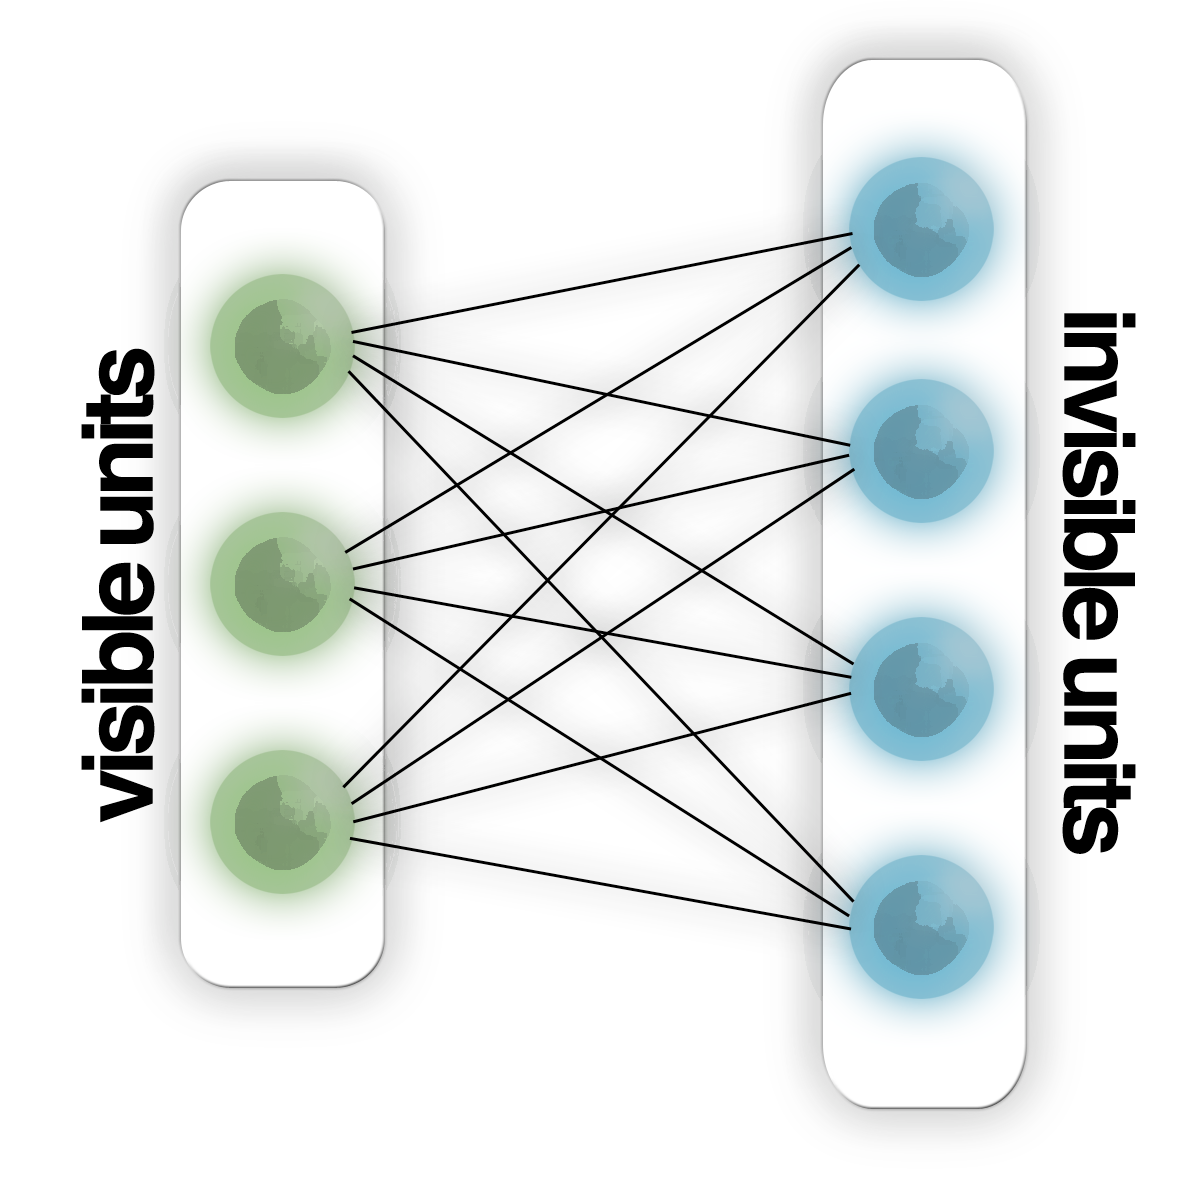
\includegraphics{RBM-1.eps}}
  \caption{Restricted Boltzmann Machine}
\end{figure}


The connections between the neurons in the two layers is symmetrical, so it
can be represented as a weight matrix which keeps the connection between hidden
and visible layers. A state of a Restricted Boltzmann machine is given by the
values of both the visible and given state. The corresponding Hopfield energy
formula for a state is given by :
\[ E (v, h) = - \sum_{i \in V} a_i v_i - \sum_{j \in H} b_j h_i - \sum_{i \in
   V, \nocomma j \in H \nocomma} v_i h_j w_{\tmtextit{\tmtextit{\tmop{ij}}}}
\]


where, $w_{\tmtextit{\tmtextit{}}}$is the weight matrix, $a$ and $b$are the
vectors of biases corresponding to the visible, respectively hidden layers. As
expected, $v$is vector of visible units and \tmtextit{h} is the vector of
hidden units.

We denote by \tmtextit{V} = \{1, .. \tmtextit{length} \tmtextit{v}\} , the
indices of a visible vector and by \tmtextit{H} = \{1, .. \tmtextit{length}
\tmtextit{h}\} the indices of a hidden vector.



\subsection{Probability of a state}

After traning, the network assigns a probability to each possible state, as
follows:
\[ p \left( v, h \right) = \frac{1}{Z} e^{- E \left( v, h \right)} \]
where Z is used to normalize the probabilities
\[ Z = \sum_{v, h} e^{- E \left( v, h \right)} \]
Thus, the probability the network asessings for a visibile vector \tmtextit{v}:
\begin{equation}
  p \left( v \right) = \sum_h \frac{1}{Z} e^{- E \left( v, h \right)}
\end{equation}

\subsection{Training the network}

The network can be trained such that one maximizes the probability of a training
pattern. The derivative of the log probability of a training vector (given by
(1)), is simple, as follows:
\[ \frac{\delta \log p \left( v \right)}{\delta w_{\tmop{ij}}} = < v_i h_i
   >_{\tmop{data}} - < v_i h_i >_{\tmop{model}} \]
Due to the fact that the Restricted Boltzmann Machine can be represented as a bipartite graph, it is easy
to attain an \tmtextit{unabiased} sample of the hidden units, given the
visible units.
\begin{equation}
  p \left( h_j = 1 \left|  \right. v \right) = \sigma \left( b_j + \sum_{i \in
  V} v_i w_{\tmop{ij}} \right)
\end{equation}
For the visible units, the same formula gives a \tmtextit{biased} sample of
the visible units.
\begin{equation}
  p \left( v_i = 1 \left|  \right. h \right) = \sigma \left( a_i + \sum_{j \in
  H} h_j w_{\tmop{ij}} \right)
\end{equation}


where $\sigma = \frac{1}{1 \noplus + e^{- x}}^{}$, is the logistic sigmoid
function.

There are ways of getting an unbiased sample of the visible units, but they
are very time consuming. In practice, the contrastive divergence algorithm is
used as a faster substitute. The visible units are set to a training vector
and the binary states of the hidden vector are computed using (2). These
binary units are used to \tmtextit{reconstruct} the states of the visible
vector using (3).

The training rule then becomes:
\[ \Delta w_{\tmop{ij}} = \lambda \left( < v_i h_i >_{\tmop{data}} - < v_i h_i
   >_{\tmop{reconstruction}} \right) \]
We note that the above training rule has the desired properties for modeling
the biological brain: it is both \tmtextit{local} and \tmtextit{incremental}.
Angle brackets \ denote the expected value under the given distribution by the
following subscript.



\subsection{Using Restricted Boltzmann Machines for classification}

As suggested by Hinton in section 16 \cite{hinton2010practical}, there are various ways of using Restricted
Boltzmann Machines for classification. We have employed two methods, one which
we developed ourselves and another one described in the paper. The latter is adding
another set of visible units, called the \emph{classification units}.



\ \ \ \ \ \ \ \ \ \ \ \ \ \ \ \ \ \ \ \ \ \ \ \begin{figure}[h]
  \ \ \ \ \ \ \ \ \ \ \centering
  \resizebox{350px}{350px}{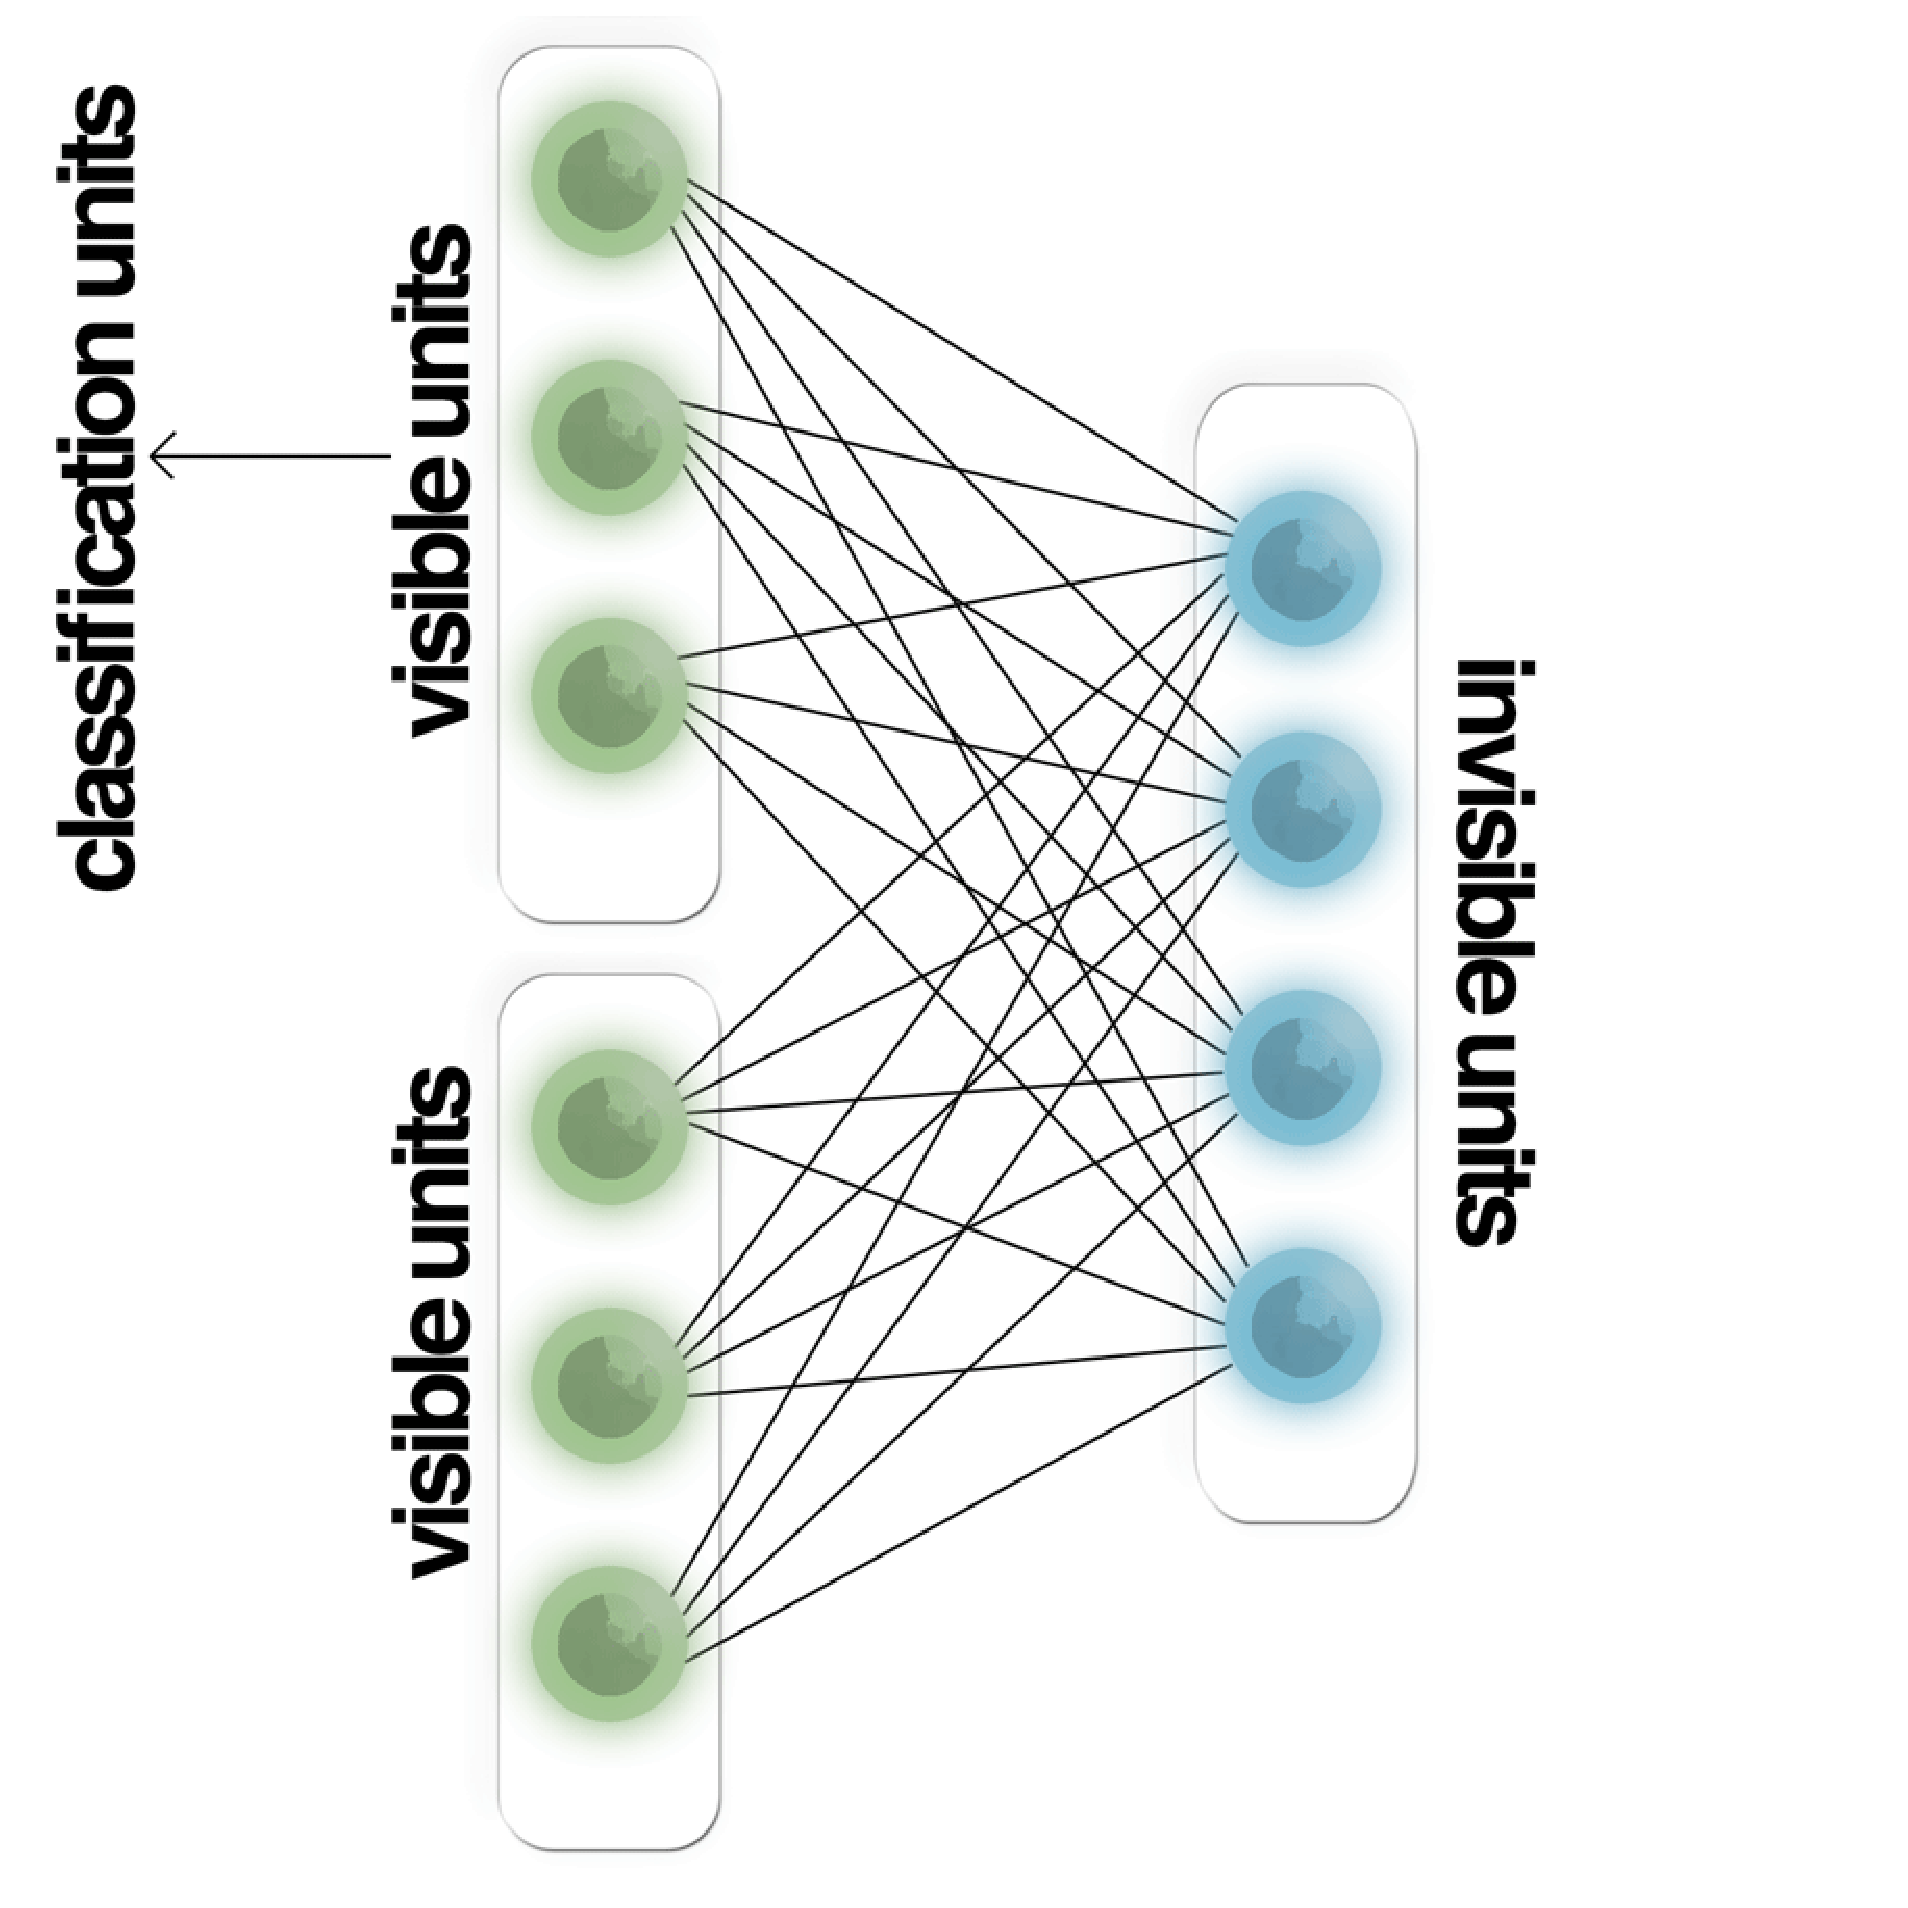
\includegraphics{RBM-2.eps}}
  \caption{Classification Boltzmann machine}
\end{figure}



The vector of hidden units is used to model the joint distribution between a
vector of inputs v and a target (classification) vector y. The classification
vector y corresponds to a class. It's length is given by the number of
classes. $y = e_c$, where c is the class the vector is modeling ($e_c$ is a
vector with all zeros, expect from the position c, where it is 1).

As seen from Figure 2, one now needs to weight matrices, which we will denote
by \tmtextit{W}(the weight matrix between the visible units and hidden ones) \
and U (the weight matrix and between the classification units and hidden
ones). Vectors \tmtextit{b}, \tmtextit{c}, \tmtextit{d} correspond to the
vector of biases for the visible units (training patterns), hidden units and
classification units, respectively.

The energy function for this model is:
\[ E \left( v \nocomma, y, h \right) = - d^T y - c^T h - b^T v - h^T W v - h^T
   U y \]
Which gives rise to the following formula for the probability of a configuration
\tmtextit{v}, \tmtextit{y}.
\[ p \left( v, y, h \right) = \frac{e^{- E \left( v \nocomma, y, h
   \right)}}{Z} \]
where \tmtextit{Z} is the normalizing constant. Thus,
\[ p \left( v, y \right) = \sum_h p \left( v, y, h \right) = \sum_h \frac{e^{-
   E \left( v \nocomma, y, h \right)}}{Z} \]
The distribution used for the Classification Boltzmann Machine are the
following:
\begin{equation}
  p \left( h_i = 1 \left| v, y \right. \right) = \sigma \left( c_j + \noplus
  \noplus W_j v \noplus + U_j y \right)
\end{equation}
\begin{equation}
  p \left( v_i = 1 \left| h \right. \right) = \sigma \left( b_j + \noplus
  \noplus h^T W^i  \right)
\end{equation}
\begin{equation}
  p \left( y = e_c \left| h \right. \right) = \frac{e^{d^T e_c \noplus + h^T
  Ue_c}}{N}
\end{equation}
where N is the normalizing constant $\sum_c$ $e^{d^T e_c \noplus + h^T Ue_c}$.

Note that we denote by $W_i$ the row \tmtextit{i} of matrix \tmtextit{W}, and
by $W^i_{}$ the column \tmtextit{i} of matrix \tmtextit{W}.



Valuable reference for this was given to us from
\cite{louradour2011classification} and
\cite{larochelle2008classification}.

\subsection{Learning}

Contrastive divergence can be used to train the network, giving rise to the
following update rules:


\begin{eqnarray*}
  b'  & = & b + \lambda \left( v - v_{\tmop{sampled}} \right)\\
  c'  & = & c + \lambda \left( h_{\sigma} - h_{\sigma \tmop{sampled}}
  \right)\\
  d'  & = & d + \lambda \left( y - y_{\tmop{sampled}} \right)\\
  W'  & = & W + \lambda \left( h_{\sigma} v^T - h_{\sigma \tmop{sampled}}
  v_{\tmop{sampled}}^T \right)\\
  U' & = & U + \lambda \left( \left. h_{\sigma} y^T - h_{\sigma
  \tmop{sampled}} y_{\tmop{sampled}}^T \right) \right.
\end{eqnarray*}
where we denote by $x'$ the new value of parameter x. $v_{\tmop{sampled}} $and
$y_{\tmop{sampled}} $are obtained by sampling the distributions in (5) and
(6).
\begin{eqnarray*}
  h_{\sigma} & = & \sigma \left( c_j + \noplus \noplus W_j v \noplus + U_j y
  \right)\\
  h_{\sigma \tmop{sampled}} & = & \sigma \left( c_j + \noplus \noplus W_j
  v_{\tmop{sampled}} \noplus + U_j y_{\tmop{sampled}}  \right)
\end{eqnarray*}
\subsection{Classification}
\[ p \left( y = e_c \left| v \right. \right) = \frac{e^{- F \left( v \nocomma,
   e_c \right)}}{\sum_d e^{- F \left( v \nocomma, e_d \right)}} \]
where $F \left( v \nocomma, e_c \right) $is the \tmtextit{free energy
function}
\[ F \left( v \nocomma, e_c \right) = - d^T y - \sum^H_{j = 1}
   \tmtextit{\tmtextit{s}} \left( c_j + \noplus \noplus W_j v \noplus + U_j y
   \right) \nocomma \]
where $s \left( x \right) = \log \left( 1 + e^x \right) $



The implementation of the Classification Boltzmann Machine can be found in

\tmtexttt{ClassficationBoltzmannMachine.hs. }



\subsection{New method}

Another method we have employed using Boltzmann Machines was created by us. We
have never seen this approach used somewhere else. Instead of creating 2 types
of visible units, we use the simple Restricted Boltzmann Machine, with one
type of visible units (and hence a single matrix). For each training vector
we append the classification at the end. The classification is represented as
a binary vector, either as above, by using $e_c$, where c is the
classification of the current pattern, or even in a more compressed manner, by
creating the binary vector using the representation in base 2 of class c.

\ \ \ \ \ \ \ \ \ \ \ \ \ \ \ \ \ \ \ \ \ \ \ \ \ \ \ \ \ \ \ \ \ \ \ \ \ \
\ \ \

\ \ \ \ \ \ \ \ \ \ \ \ \ \ \ \ \ \ \ \ \ \ \ \ \ \ \ \ \ \ \ \ \ \ \ \ \

\ \ \ \ \ \ \ \ \ \ \ \ \ \ \ \ \ \begin{figure}[h]
  \ \ \ \ \ \ \ \ \ \ \ \ \
  \centering
  \resizebox{350px}{350px}{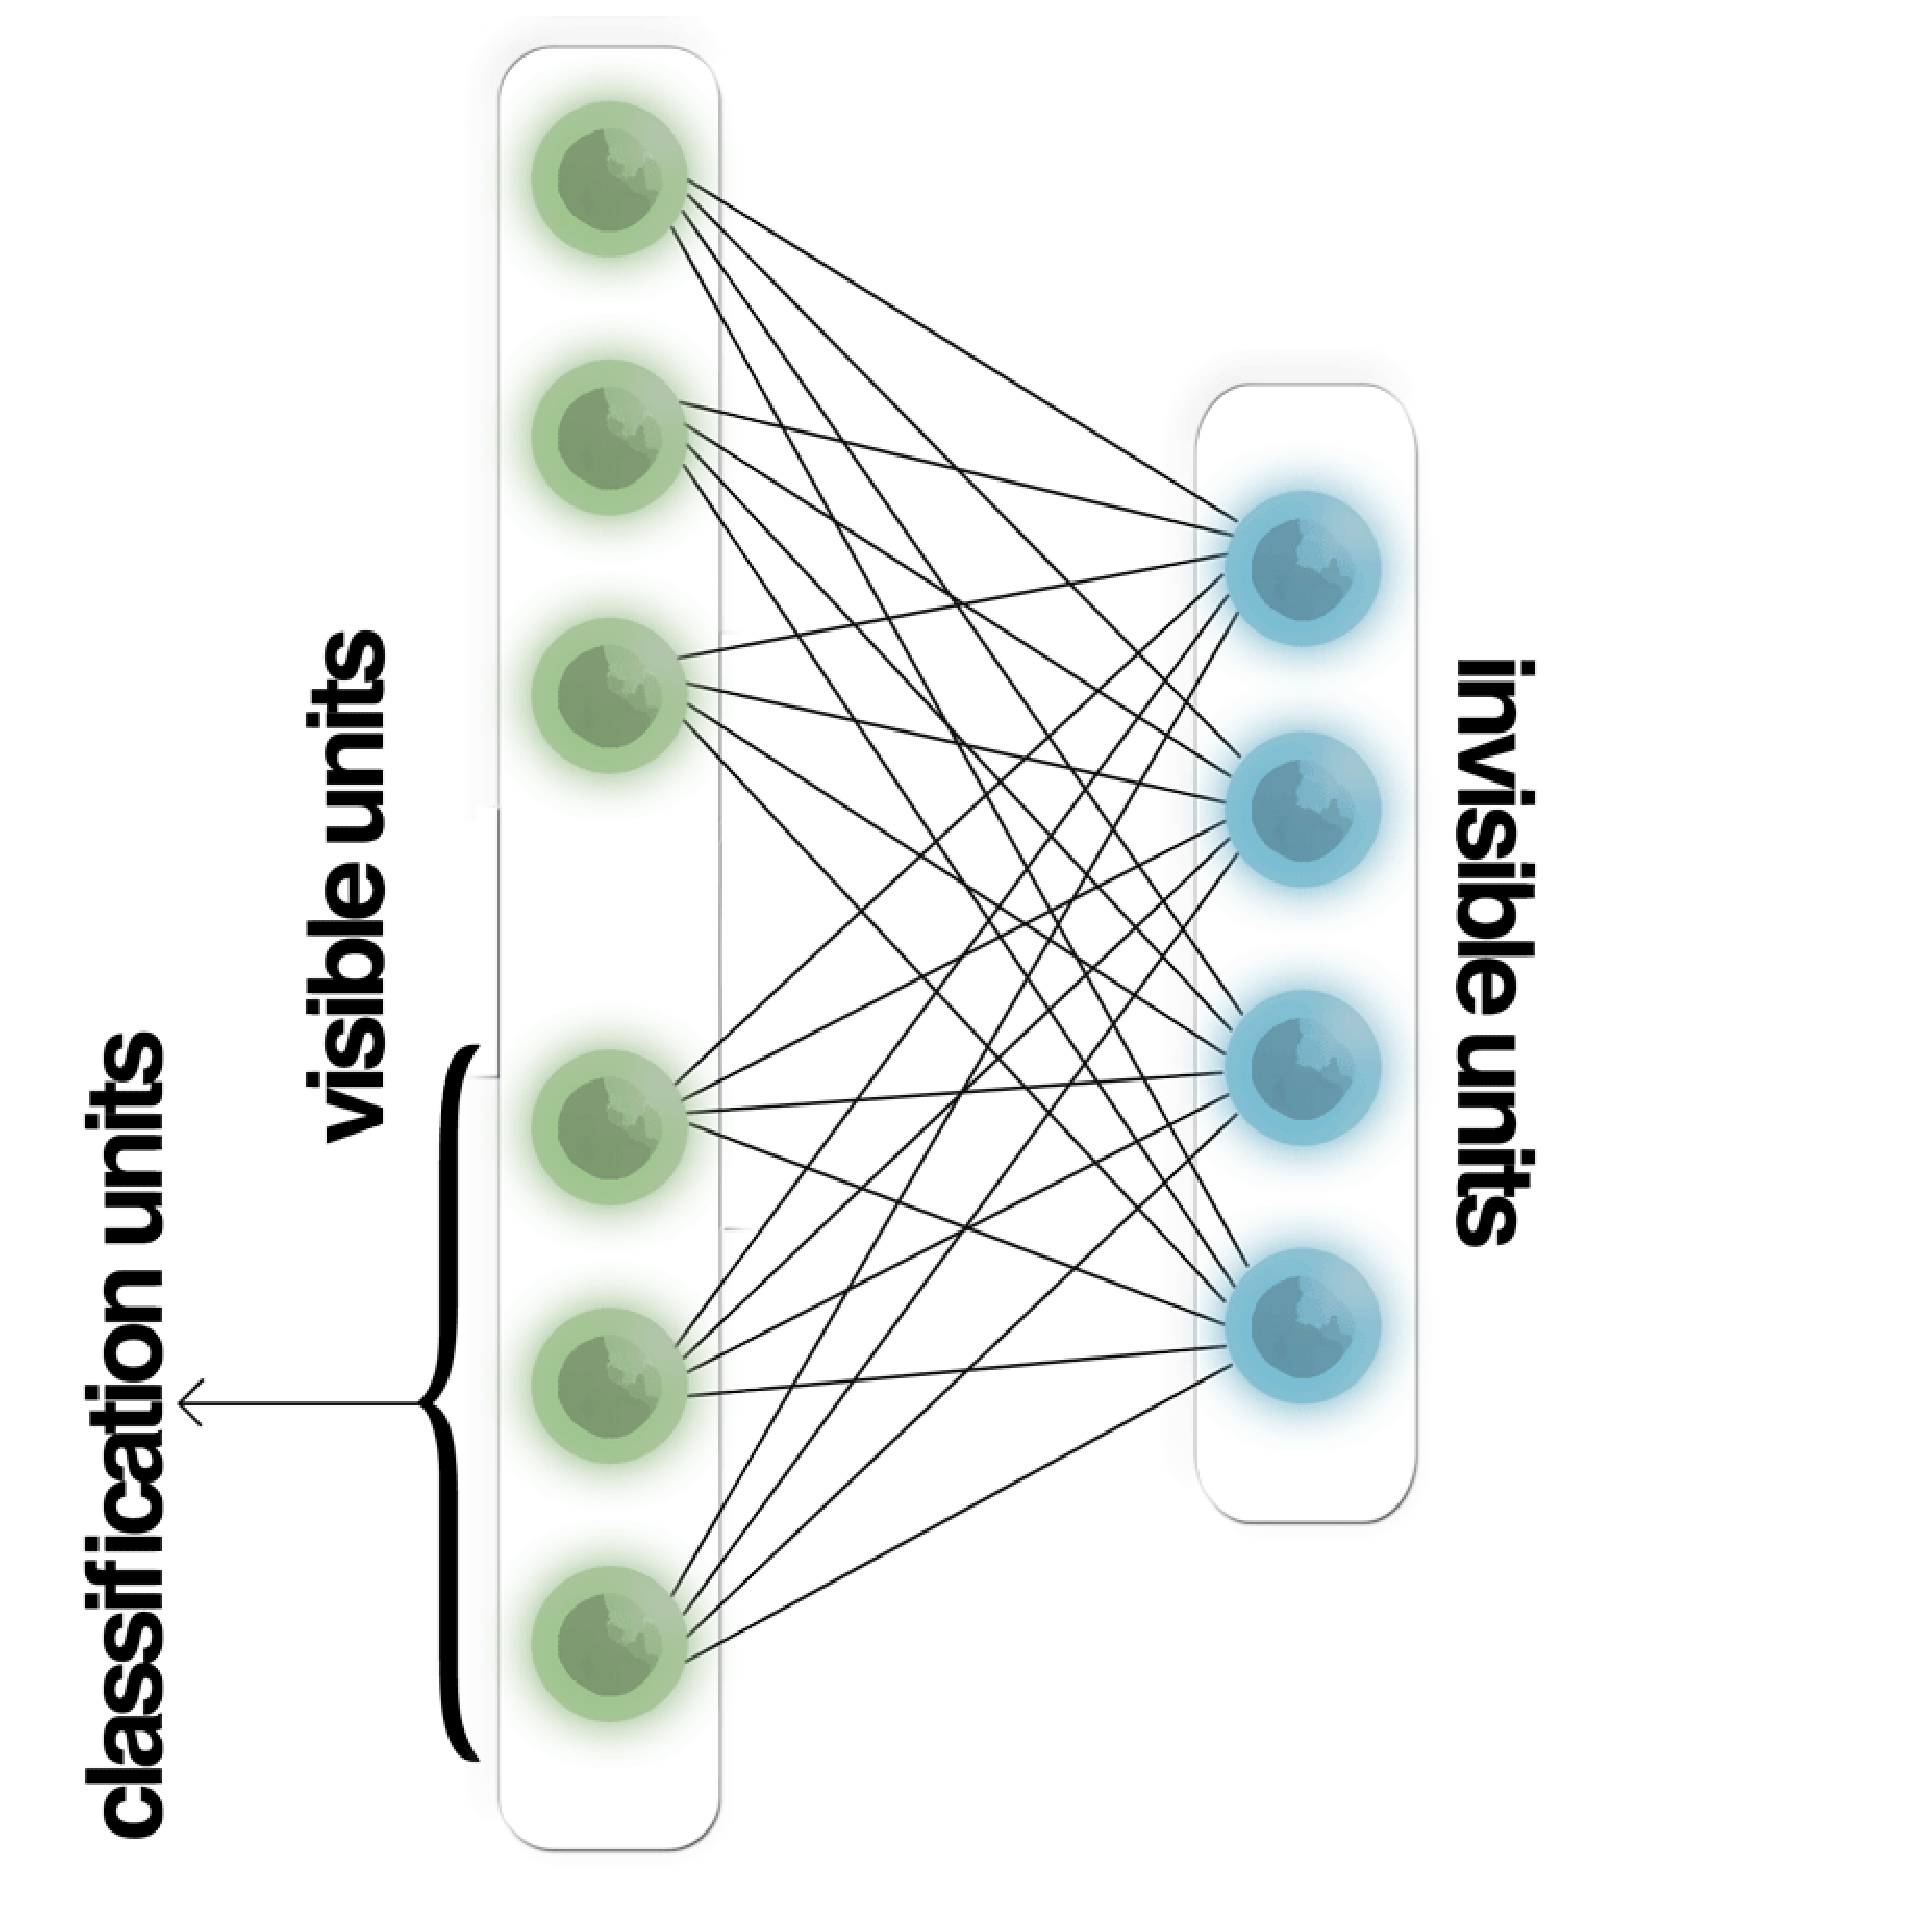
\includegraphics{RBM-3.eps}}
  \caption{Boltzmann machines according to our new method}
\end{figure} \ \ \ \ \ \ \ \ \ \ \ \ \ \ \ \ \ \ \ \ \ \ \ \ \ \ \ \ \ \ \ \ \
\ \ \ \ \ \

\ \ \ \ \ \ \ \ \ \ \ \ \ \ \ \ \ \ \ \ \ \ \ \ \ \ \ \ \ \ \ \ \ \

The training is done in the usual way, but with the complete vectors (actual
pattern and classification). In our case, as different patterns ought to have
different classifications, we use as class the index of the pattern in the list
(with removed duplicates) of training patterns.

When a pattern needs to be matched to one of the training patterns for
recognition, one uses the log probability (given using ...) to compute the
probability of each of the classifications, and choses the one with maximum
probability.



\begin{figure}[h]
  \centering
  \resizebox{622px}{182px}{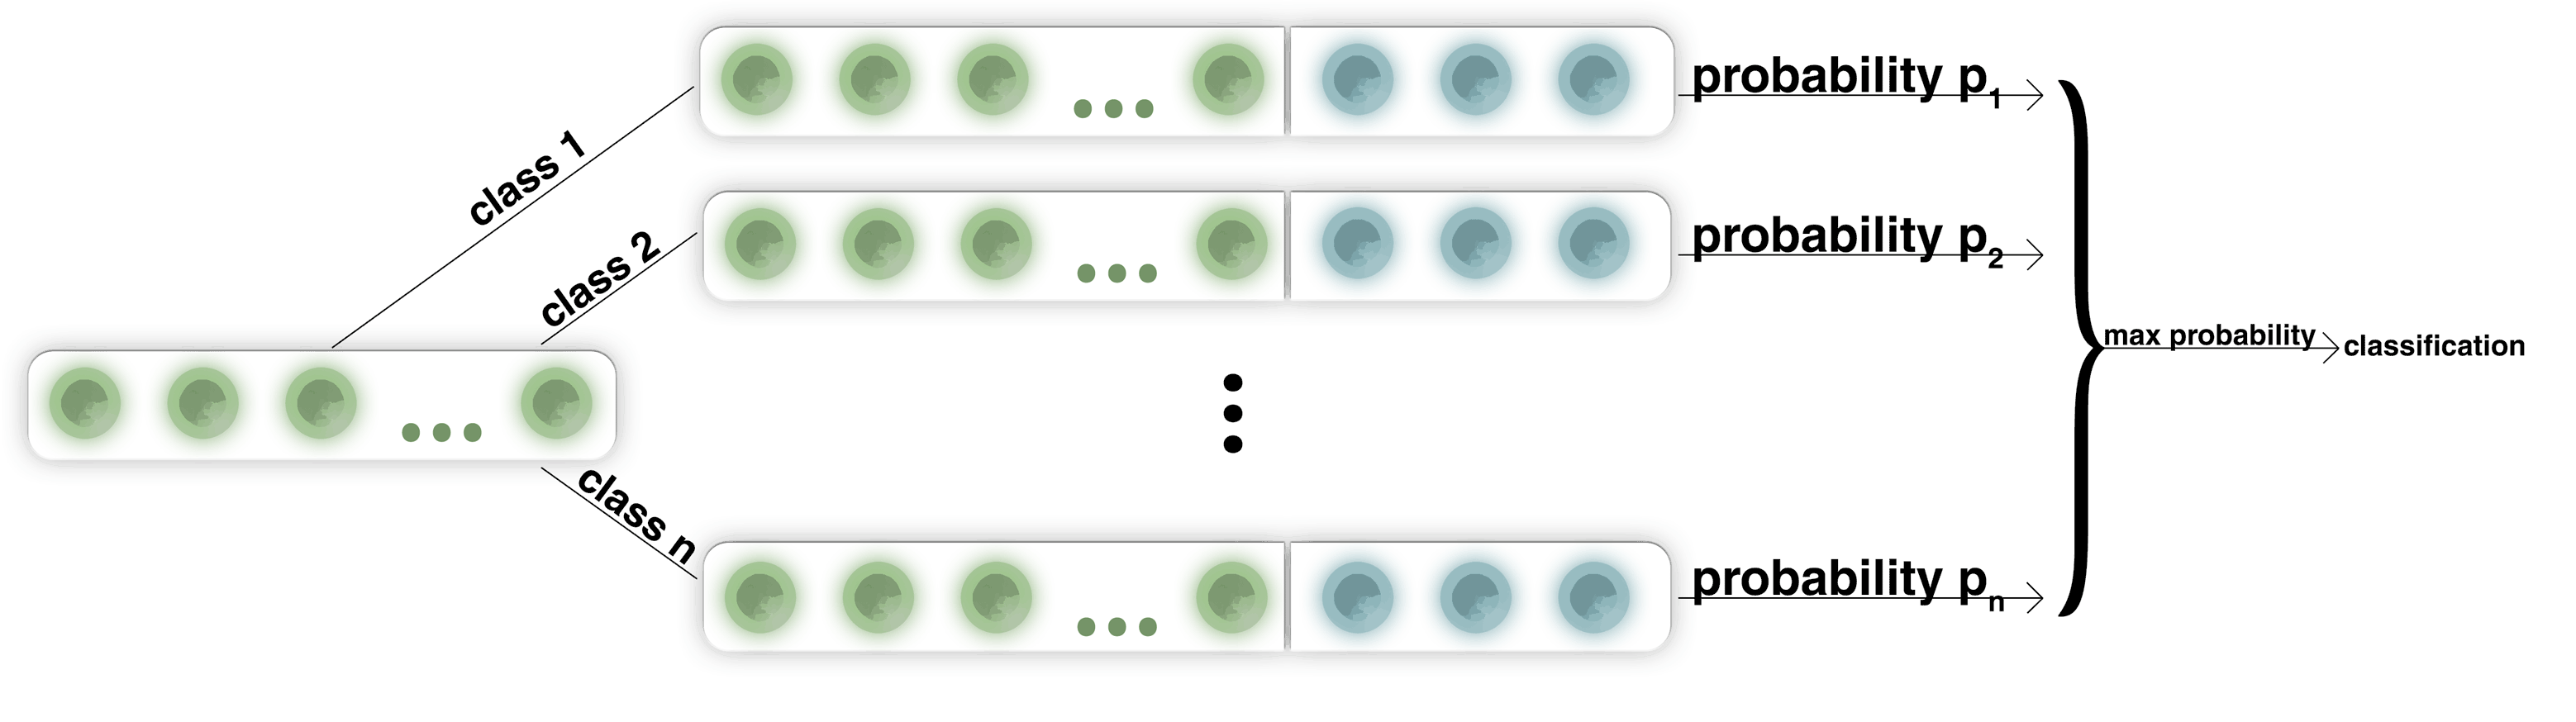
\includegraphics{RBM-4.eps}}
  \caption{The recognition process in the new Boltzmann machine.}
\end{figure}



As given in \cite{hinton2010practical}, the log
probability is  given by:
\[ \tmtextit{\log} \left( \tmop{class} = c \left| v \right. \right) =
   \frac{e^{- F_c \left( v \right)}}{\sum_{c'} e^{- F_{c'} \left( v
   \right)}} \]
\[ F \left( v \right) = - \sum_{i \in V} v_i a_i - \sum_{j \in H} \log \left(
   1 \noplus + e^{x_j} \right) \]


where $x_j = b_j + \sum_i w_{ij_{}} v_j$



The implementation of this procedure can be found in
\tmtexttt{RestrictedBoltzmannMachine.hs.}



% undefined variables
\let\psuper\undefined
\let\prandom\undefined
